\documentclass{standalone}
\usepackage{tikz}
\usepackage{ctex,siunitx}
\usepackage{tkz-euclide}
\usepackage{amsmath}
\usetikzlibrary{patterns, calc}
\usetikzlibrary {decorations.pathmorphing, decorations.pathreplacing, decorations.shapes,}
\begin{document}
\small
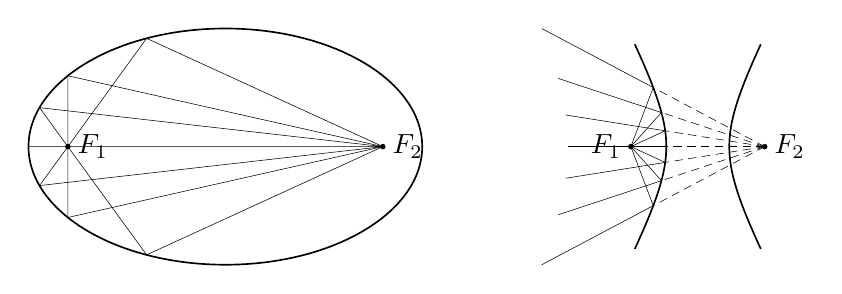
\begin{tikzpicture}[>=latex,scale=0.5]
  \begin{scope}
    \draw[semithick](0,0)ellipse(5 and 3);
    \draw[very thin](4,0)--(-4,1.8)--(-4,-1.8)--cycle;
    \draw[very thin](4,0)--(-2,2.7495)--(-4.72,-0.9898)--cycle;
    \draw[very thin](4,0)--(-2,-2.7495)--(-4.72,0.9898)--cycle(4,0)--(-5,0);
    \fill (4,0)circle(2pt)node[right]{$F_2$};
    \fill (-4,0)circle(2pt)node[right]{$F_1$};
  \end{scope}
  \begin{scope}[xshift=12cm]
    \draw[semithick,samples=200,domain=-60:60] plot ({0.8/cos(\x)},{1.5*tan(\x)});
    \draw[semithick,samples=200,domain=-60:60] plot ({-0.8/cos(\x)},{1.5*tan(\x)});
    \foreach \x in {-45,-30,-15,0,15,30,45}
    {
      \draw[very thin,densely dashed](1.7,0)--({-0.8/cos(\x)},{1.5*tan(\x)});
      \draw[very thin](-1.7,0)--({-0.8/cos(\x)},{1.5*tan(\x)})--++({-0.8/cos(\x)-1.7},{1.5*tan(\x)});
    }
    \fill (1.7,0)circle(2pt)node[right]{$F_2$};
    \fill (-1.7,0)circle(2pt)node[left]{$F_1$};
  \end{scope}
\end{tikzpicture}
\end{document}